% Latex Template
%
% Fall 2015
%
% Andy Sayler

\documentclass[11pt,twocolumn,letterpaper]{article}

% System Packages
\usepackage{epsfig}
\usepackage{float}
\usepackage{caption}
\usepackage{subcaption}
\usepackage{tabu}
\usepackage{color}
\usepackage{hyperref}
\usepackage{url}

% Local Packages
% None

% Package Options
\hypersetup{
    colorlinks,
    citecolor=black,
    filecolor=black,
    linkcolor=black,
    urlcolor=black
}

% Macros
\newenvironment{packed_enum}{
\begin{enumerate}
  \setlength{\itemsep}{1pt}
  \setlength{\parskip}{0pt}
  \setlength{\parsep}{0pt}
}{\end{enumerate}}

\newenvironment{packed_item}{
\begin{itemize}
  \setlength{\itemsep}{1pt}
  \setlength{\parskip}{0pt}
  \setlength{\parsep}{0pt}
}{\end{itemize}}

\newenvironment{packed_desc}{
\begin{description}
  \setlength{\itemsep}{1pt}
  \setlength{\parskip}{0pt}
  \setlength{\parsep}{0pt}
}{\end{description}}


% Other Options
\clubpenalty = 10000
\widowpenalty = 10000

% Start
\begin{document}

\title{Example Document}
% Subtitles aren't supported in the ``article'' document class, but if
% they were, you could add one via the following line.
%\subtitle{Example Document}

\author{Example Author}

\maketitle

\begin{abstract}
This is an example \LaTeX document. This is its abstract. Give the
reader an overview of the document here.
\end{abstract}

\section{Section 1}
\label{sec:section1}

This is an example section.

\subsection{Subsection A}
\label{sec:section1A}

This is an example subsection

\section{Section 2}
\label{sec:section2}

This is another section.

\noindent
This is a citation~\cite{exampleref1}.

% The tilde (~) in the previous sentence is optional, and just helps
% to insure citations and references don't wind up on a new line
% separated from the text they're attached to.

% noindent can be used to prevent indentation on single-line paragraphs.

\begin{figure}[htb]
  \centering
  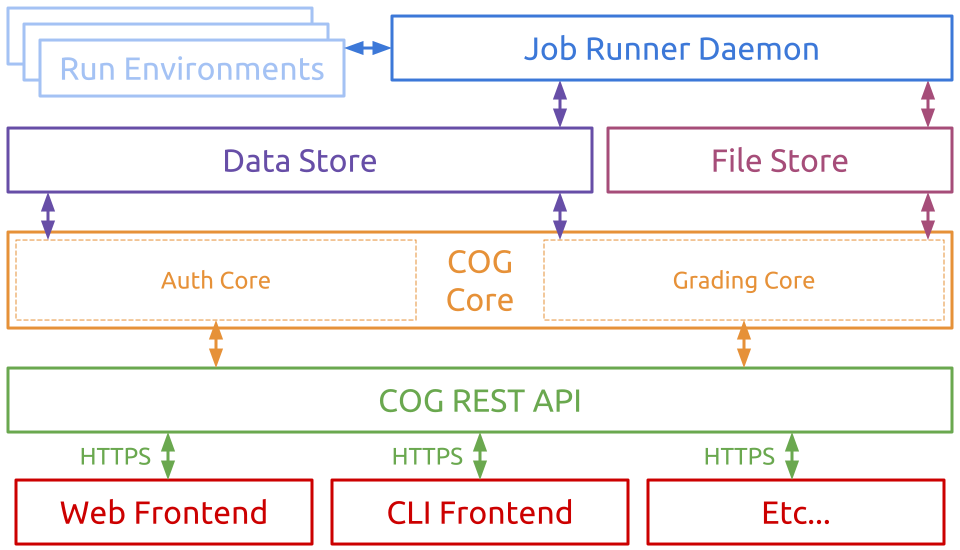
\includegraphics[width=\columnwidth]{./figs/pdf/examplefig1.pdf}
  \caption{Example Figure 1}
  \label{fig:example1}
\end{figure}

\noindent
Figure~\ref{fig:example1} is an example figure. The proceeding
sentence contains a reference to it.

\noindent
Sometimes you want thing in {\bf bold}.

\noindent
Or in {\em italics}.

\noindent
Or in \texttt{type-write font}.

\noindent
Sometime you need to do some math: $9/3=3$.

\noindent
Or ``a quote.''

\noindent
Or add a bullet list:

\begin{packed_item}
\item Item A
\item Item B
\item Item C
\end{packed_item}

\noindent
Or a numbered list:

\begin{packed_enum}
\item Item 1
\item Item 2
\item Item 3
\end{packed_enum}

\noindent
Or a definitions list:

\begin{packed_desc}
\item[Item I:] This is item 1 
\item[Item II:] This is item 2
\item[Item III:] This is item 3
\end{packed_desc}

% Note: The ``packed'' variants of the above items are my own and are
% defined in macros.tex. They are more tightly spaced versions of the
% standard LaTeX enumerate, itemize, and description environments.

\bibliographystyle{acm}
\bibliography{refs}

\end{document}
